%%%%%%%%%%%%%%%%%%%%%%%%
%% Sample use of the infthesis class to prepare a thesis. This can be used as
%% a template to produce your own thesis.
%%
%% The title, abstract and so on are taken from Martin Reddy's csthesis class
%% documentation.
%%
%% MEF, October 2002
%%%%%%%%%%%%%%%%%%%%%%%%

%%%%
%% Load the class. Put any options that you want here (see the documentation
%% for the list of options). The following are samples for each type of
%% thesis:
%%
%% Note: you can also specify any of the following options:
%%  logo: put a University of Edinburgh logo onto the title page
%%  frontabs: put the abstract onto the title page
%%  deptreport: produce a title page that fits into a Computer Science
%%      departmental cover [not sure if this actually works]
%%  singlespacing, fullspacing, doublespacing: choose line spacing
%%  oneside, twoside: specify a one-sided or two-sided thesis
%%  10pt, 11pt, 12pt: choose a font size
%%  centrechapter, leftchapter, rightchapter: alignment of chapter headings
%%  sansheadings, normalheadings: headings and captions in sans-serif
%%      (default) or in the same font as the rest of the thesis
%%  [no]listsintoc: put list of figures/tables in table of contents (default:
%%      not)
%%  romanprepages, plainprepages: number the preliminary pages with Roman
%%      numerals (default) or consecutively with the rest of the thesis
%%  parskip: don't indent paragraphs, put a blank line between instead
%%  abbrevs: define a list of useful abbreviations (see documentation)
%%  draft: produce a single-spaced, double-sided thesis with narrow margins
%%
%% For a PhD thesis -- you must also specify a research institute:
%\documentclass[phd,ilcc,twoside]{infthesis}

%% For an MPhil thesis -- also needs an institute
% \documentclass[mphil,ianc]{infthesis}

%% MSc by Research, which also needs an institute
% \documentclass[mscres,irr]{infthesis}

%% Taught MSc -- specify a particular degree instead. If none is specified,
%% "MSc in Informatics" is used.
 %%\documentclass[mscres,ianc,draft,logo]{infthesis}
 \documentclass[mscres,ianc,abbrevs]{infthesis}
% \documentclass[msc]{infthesis}  % for the MSc in Informatics

%% Master of Informatics (5 year degree)
% \documentclass[minf]{infthesis}

%% Undergraduate project -- specify the degree course and project type
%% separately
% \documentclass[bsc]{infthesis}
% \course{Artificial Intelligence and Psychology}
% \project{Fourth Year Project Report}

%% Put any \usepackage commands you want to use right here; the following is 
%% an example:
%%\usepackage{natbib}
\usepackage[pdftex]{graphicx}
\usepackage{amsmath}
\usepackage{amssymb}
\usepackage{relsize}
\usepackage{subfigure}
\usepackage{float}
\usepackage{multirow}
\usepackage{bm}
\usepackage{bbm}
\usepackage{tikz}
\definecolor{darkblue}{rgb}{0.0, 0.0, 0.6}
\usetikzlibrary{positioning}
\usetikzlibrary{bayesnet}
\usepackage[colon,authoryear]{natbib}
\usepackage[pdftex,
            pagebackref=false,
            colorlinks=true,
            linkcolor=black,
	    	citecolor=darkblue,
	    	filecolor=black,
	    	urlcolor=black,
            unicode
            ]{hyperref}
%\hypersetup{
%     colorlinks   = true,
%     citecolor    = darkblue
%}

\newcommand{\bigCI}{\mathrel{\text{\scalebox{1.07}{$\perp\mkern-10mu\perp$}}}}

%% Information about the title, etc.
\title{Integrative Clustering of Multisource Biomedical Data}
\author{Chantriolnt - Andreas Kapourani}

%% If the year of submission is not the current year, uncomment this line and 
%% specify it here:
% \submityear{1785}

%% Optionally, specify the graduation month and year:
% \graduationdate{February 1786}

%% Specify the abstract here.
\abstract{%
Abstract goes here...
}

%% Now we start with the actual document.
\begin{document}

%% First, the preliminary pages
\begin{preliminary}

%% This creates the title page
\maketitle

%% Acknowledgements
\begin{acknowledgements}
Acknowledgements go here ...
\end{acknowledgements}

%% Next we need to have the declaration.
\standarddeclaration

%% Finally, a dedication (this is optional -- uncomment the following line if
%% you want one).
%%\dedication{to my mummy}

%% Create the table of contents
\tableofcontents

%% If you want a list of figures or tables, uncomment the appropriate line(s)
\listoffigures
\listoftables

\end{preliminary}

%%%%%%%%
%% Include your chapter files here. See the sample chapter file for the basic
%% format.

\chapter{Introduction} \label{introduction-ch}

\section{Motivation} \label{motivation-intro-l}

\section{Outline} \label{outline-intro-l}
The rest of this document is organized as follows: ...

\chapter{Background} \label{background-chapter}

%\section{Molecular Biology Background} \label{molecular-back-sect}
Epigenetics is a relatively new scientific field in Molecular Biology, and it describes the study of dynamic alterations in the transcriptional regulation of a cell. We can think of the epigenome as an external layer of information onto the genomic sequence, which can be used to understand major cellular processes, such as transcription, splicing and replication \citep{Furey2012}.

Regulation of gene expression in higher eukaryotic organisms depends on sequences within the DNA itself known as \emph{promoters}, and on a network of regulatory proteins, called \emph{transcription factors} (TFs) \citep{Jasny2001}. TFs are proteins that bind to specific DNA sequences, which are associated with specific genes, and facilitate of inhibit the recruitment of RNA polymerase in the promoter region of those genes \citep{Ptashne2002}. 

Recent advances in epigenetics have suggested some other mechanisms that regulate gene expression, such as the changes of the accessibility of the DNA, e.g. \emph{histone modifications} (HMs), and \emph{DNA methylation}. Histones are proteins that act as a spool where DNA can be wrapped around them to form \emph{nucleosomes}. The combination of DNA and nucleosomes within the nucleus of eukaryotic cells is called the \emph{chromatin}. 

DNA methylation is an epigenetic mark which occurs when a methyl group is attached to the \emph{cytosine} DNA nucleotides. In mammals, which we are mostly interested in this project, DNA methylation is observed almost exclusively on cytosines in the context of CpG dinucleotides (i.e. C followed by G, where p stands for the phosphate group between C and G). Genome wide CpGs are depleted, but mainly near promoter regions there are clusters of CpGs, which are called CpG islands (CGIs) \citep{Bird2002}. 

Owing to the rapid development of Next Generation Sequencing (NGS) technology, it is reasonable to expect genome sequences and other forms of high-throughput data to be measured extensively. For example, \emph{RNA-Seq} experiments \citep{Wang2009} are widely used for transcriptome profiling, i.e. measuring the set of all RNA molecules produced in a given cell or cell population (at a given time). \emph{Chip-Seq} experiments \citep{Park2009} are used to quantitatively measure and analyse protein interactions with DNA, i.e. HMs and binding of TFs. Whole-Genome Bisulphite Sequencing (WGBS) \citep{Frommer1992}, and Reduced Representation Bisulphite Sequencing (RRBS) \citep{Meissner2008}, are methods that use bisulphite treatment of DNA and allow estimation of methylation proportions at a single-nucleotide resolution. These are only some examples of the different platforms and techniques that are used to measure diverse biological components and are shown in \emph{Fig. \ref{seq-pic}}. 

\begin{figure}[h]
\begin{center}
 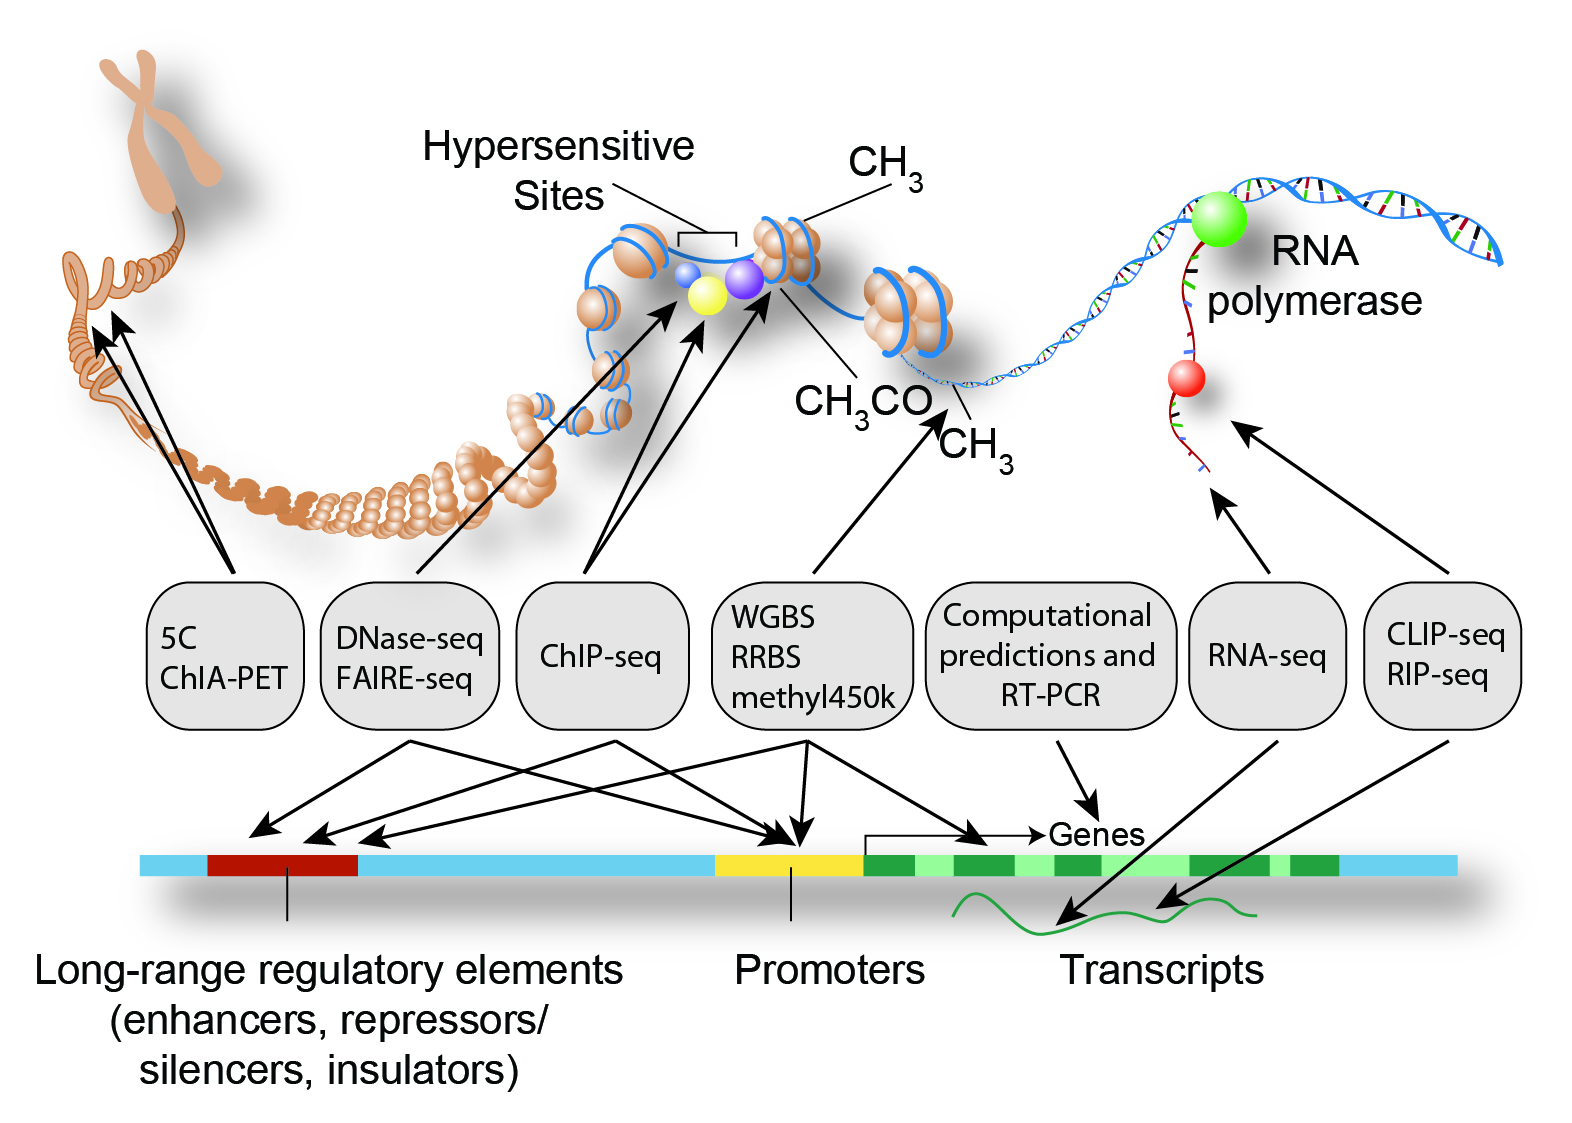
\includegraphics[scale = 0.15]{images/encode-seq.png}
\caption{\emph{Some of the XX-Seq techniques used from the ENCODE projet. Credits: Darryl Leja (NHGRI), Ian Dunham (EBI), Michael Pazin (NHGRI) \citep{Dunham2012}.}}
\label{seq-pic}
\end{center}
\end{figure} 

Recent research studies, assisted by whole-genome data analysis, demonstrated that gene expression and histone modifications (HMs) are well correlated, since a probabilistic model was created, which given a small number of HMs it could predict gene expression \citep{Karlic2010}. Also, \citep{Benveniste2014}, using the richness of the ENCODE datasets \citep{Dunham2012}, learned a logistic regression classifier with the TFs as input features and showed that only from knowledge of TF binding patterns at promoters they could accurately predict HMs. These are only some studies that show the correlation between genetic and epigenetic mechanisms. 

From the aforementioned, it is evident that in order to uncover and interpret the biological regulatory mechanisms an integrative analysis of these heterogeneous biomedical datasets should be performed, since by performing separate analyses of each data source we may not capture important associations between them.
\section{Mixture Models} \label{mixture-models-section}

The aim of this project is focused on modelling and clustering multisource biomedical data. Clustering is a widely used exploratory tool, whose main task is to identify and group similar objects together in \emph{'clusters'}. Clustering can can be categorized as an \emph{unsupervised} learning approach, since we try to discover hidden structure in unlabelled data.     

Different algorithms have been proposed for performing clustering, including hierarchical clustering (agglomerative or top down), k-means \citep{MacQueen1967}, and mixture models \citep{McLachlan1988}. This project is concentrated on \emph{mixture models} which are probabilistic, in the sense that they claim how the data might look like by modelling each cluster by certain probability density functions, \eg mixture of Gaussian distributions.  

A mixture model is a convex combination of two or more probability density functions, possibly of different distributional types. By using a superposition of the individual probability density functions, mixture models are capable of approximating any continuous distribution to arbitrary accuracy \citep{Marin2005}. Mixture models can be formulated as Latent Variable Models (LVMs), where the latent variables have discrete states and can be interpreted as defining assignments of data points to specific components of the mixture model.

Formally, let $x_{i}$, where $i \in \lbrace 1, ... , N \rbrace$, be a given dataset with N objects. The goal of clustering is to partition the objects into at most K clusters. Let $p(x_{i}|\theta)$ be the probability distribution for $x_{i}$ parametrized by $\theta$, $z_{i} \in \lbrace 1,...,K \rbrace$ represent the component that is responsible for $x_{i}$, and $\pi_{k}$ be the probability that an object belongs to cluster $k$, \ie $\pi_{k} = p(z_{i} = k)$. We refer to $\pi_{k}$ as \emph{mixing proportions} and to $z_{i}$ as \emph{latent variables} since they are not observed in the data, but are introduced to allow complicated distributions to be formed from simpler components. 

Thus, the mixture model is defined as follows:
\begin{equation} \label{mix-model-f-mm}
	\begin{aligned}
		p(x_{i}|\Theta) & = \sum_{k=1}^{K} p(z_{i} = k) p(x_{i}|\theta_{k}) \\
			& = \sum_{k=1}^{K}\pi_{k} p(x_{i}|\theta_{k})
	\end{aligned}
\end{equation}
where $\Theta = (\theta_{1},..., \theta_{k}, \pi_{1},..., \pi_{k})$ is the set of all parameters, which must satisfy:
\begin{equation}
		\pi_{k} \in (0, 1) \; \text{for} \; k \in \lbrace 1,...,K \rbrace, \; and 
\end{equation}
\begin{equation}
		\sum_{k=1}^{K}\pi_{k} = 1 
\end{equation}

Mixture models are \emph{generative models}, which means that they give us information for generating new objects. The procedure is the following: first we choose a component, with probabilities given by the mixing proportions, and then we generate an object from the corresponding probability distribution. Formally:
\begin{equation}
	\begin{aligned}
		z_{i} \; & \sim \; Cat(\pi_{1},...,\pi_{K}) \\
		x_{i} | z_{i}=k \; & \sim \; p(x_{i}|\theta_{k})
	\end{aligned}
\end{equation}
where $Cat(\pi_{1},...,\pi_{K})$ is the \emph{categorical} distribution, \ie \emph{multinomial} distribution over a single trial.

\emph{Fig.\ref{gmm-pic}} shows a Gaussian Mixture Model (GMM) with three components in two-dimensional space. It is clear that a single Gaussian distribution would be unable to capture the characteristics of the data since it is unimodal, but a linear superposition of $K$ Gaussian distributions can approximate the continuous density of the data to arbitrary accuracy. 

\begin{figure}[!ht]
	\begin{center}
 		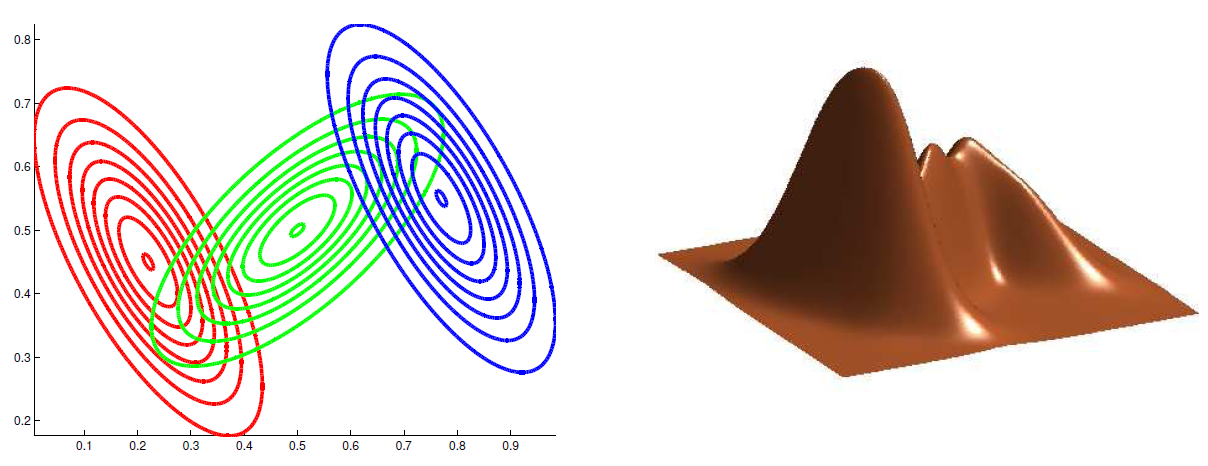
\includegraphics[scale = 0.43]{images/gmm.png}
		 	  \caption{\emph{\textbf{Left:} Contours of constant density for each of the mixture components, where each component is denoted by a different colour. \textbf{Right:} A surface plot of the probability distribution $p(\mathbf{X}|\Theta)$ \cite[Ch. \ 2]{Bishop2006}.}}
		\label{gmm-pic}
	\end{center}
\end{figure}

\subsection{Mixture Model Estimation} \label{mixt-model-estimation-l-subsect}
The model can be fitted to the data using Maximum Likelihood Estimation (MLE). The likelihood is the probability of observing the data given the parameters, and is a function of the parameters. Given a dataset $\mathbf{X}$ consisting of $N$ independent and identically distributed (i.i.d) objects $x_{1}, ..., x_{N}$, the log likelihood function for any mixture model is given by:
\begin{equation} \label{likelihood-f-mm}
	\ell(\Theta) \triangleq p(\mathbf{X}|\Theta) = \sum_{i=1}^{N} \log \bigg\lbrace \sum_{k=1}^{K}\pi_{k}p(x_{i}|\theta_{k})\bigg\rbrace
\end{equation}
The MLE approach is to find the set of parameters $\Theta$ that maximizes \emph{Eq. \ref{likelihood-f-mm}}, that is:
\begin{equation} \label{MLE-f-mm}
	\hat{\Theta} =  \underset{\Theta}{\operatorname{argmax}} \; \ell(\Theta)
\end{equation}

Unfortunately, the presence of the summation inside the logarithm in \emph{Eq. \ref{likelihood-f-mm}} prevents the possibility of deriving an analytical solution. Thus, one should use numerical optimisation procedures, and one of the most widely used algorithms for estimating parameters of mixture models is \emph{Expectation Maximization} (EM) algorithm \citep{Dempster1977}. 
\subsection{The EM algorithm} \label{em-algorithm-l-subsect}
EM is a general iterative algorithm for computing MLEs when there are missing data or latent variables. As aforementioned, mixture models can be formulated as LVMs, thus, EM arises naturally and alternates between inferring the latent values given the parameters (\emph{E-step}), and then optimizing the parameters given the filled in data (\emph{M-step}). EM exploits the fact that if the data were fully observed then the MLE would be easy to compute. In their classic paper \cite{Dempster1977} proved that EM monotonically increases the log likelihood and it converges to a maximum likelihood estimator. The algorithm ends when a convergence criterion is satisfied, \eg the log likelihood does not increase above a certain threshold between two consecutive iterations. 

\emph{Fig. \ref{em-algorithm-pic}} illustrates the EM algorithm for the mixture of two Gaussian distributions applied to the Old Faithful dataset.
\begin{figure}[ht!]
     \begin{center}
        \subfigure[]{
            \label{fig:first}
            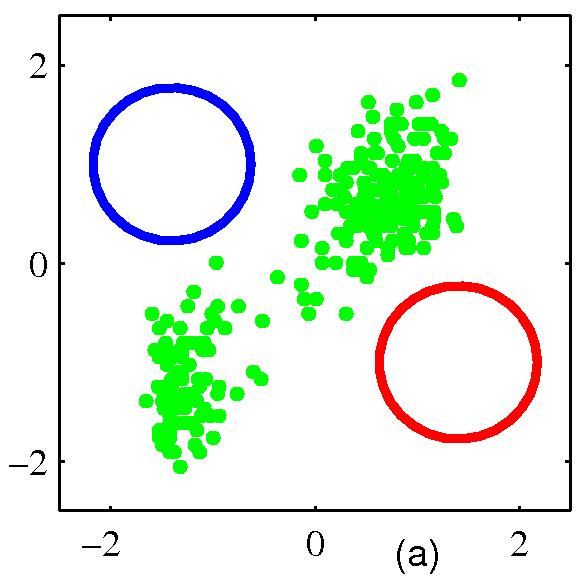
\includegraphics[width=0.3\textwidth]{images/em-a.jpg}
        }
        \subfigure[]{
           \label{fig:second}
           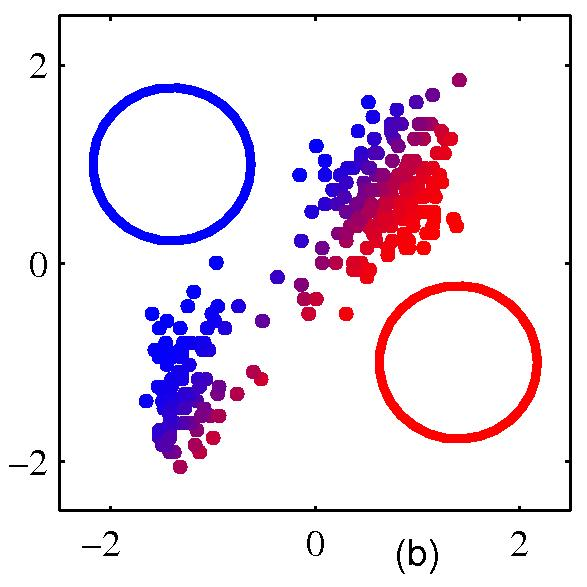
\includegraphics[width=0.3\textwidth]{images/em-b.jpg}
        }
        \subfigure[]{
            \label{fig:third}
            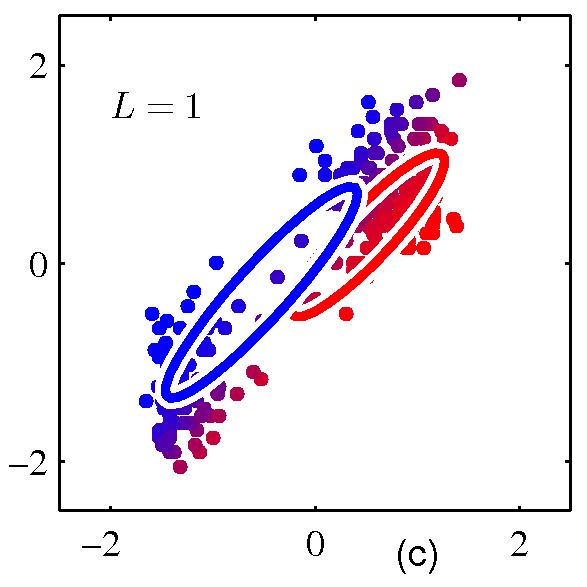
\includegraphics[width=0.3\textwidth]{images/em-c.jpg}
        } %  ------- End of the first row ----------------------%
        \subfigure[]{
            \label{fig:fourth}
            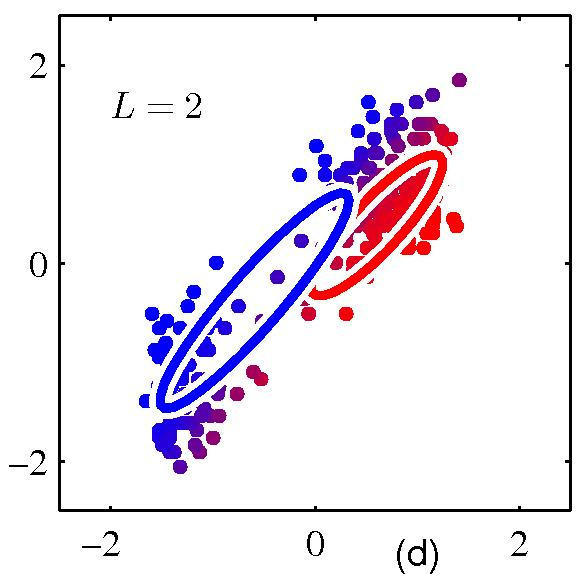
\includegraphics[width=0.3\textwidth]{images/em-d.jpg}
        }
        \subfigure[]{
            \label{fig:fifth}
            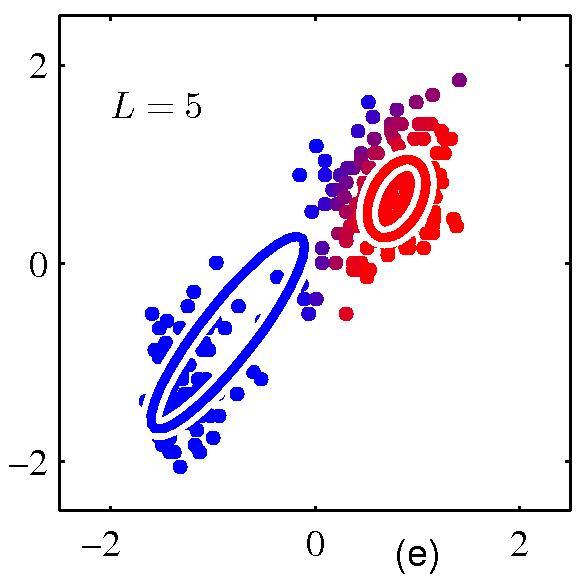
\includegraphics[width=0.3\textwidth]{images/em-e.jpg}
        }
        \subfigure[]{
            \label{fig:sixth}
            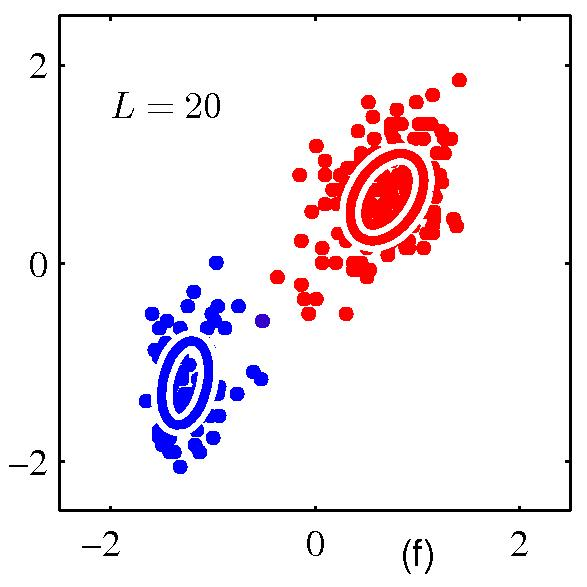
\includegraphics[width=0.3\textwidth]{images/em-f.jpg}
        }
    \end{center}
    \caption{\emph{Illustration of the EM algorithm using the Old Faithful dataset. Plot (a) shows initial parameters. Plots (b) and (c) show the E and M steps in the first iteration, respectively. Plots (d), (e) and (f) show the results after 2, 5 and 20 complete iterations of EM algorithm, respectively. \cite[Ch. \ 9]{Bishop2006}.}}
   \label{em-algorithm-pic}
\end{figure}

Our presentation for the derivation of the EM algorithm is based on \cite[Ch. \ 11]{Murphy2012}.

Let $x_{i}$ be the observed variables, and $z_{i}$ be the hidden or latent variables. We are interested in maximizing the log likelihood of the observed data:
\begin{equation} \label{log-lik-observed-f-mm}
	\ell(\Theta) \triangleq \sum_{i=1}^{N} \log p(x_{i}|\theta) =  \sum_{i=1}^{N} \log \bigg[\sum_{z_{i}} p(x_{i}, z_{i}|\theta) \bigg]
\end{equation}
which is hard to optimize due to the presence of the summation inside the logarithm, so the logarithm no longer acts directly on the likelihood function.

Let us define the \emph{complete data log likelihood} as follows:
\begin{equation} \label{log-lik-comp-observed-f-mm}
	\ell_{c}(\Theta) \triangleq \sum_{i=1}^{N} \log p(x_{i}, z_{i}|\theta)
\end{equation}

If the variables $z_{i}$ were observed, we assume that this likelihood could be easily computed. EM gets around this problem by defining the \emph{expected complete data log likelihood} as:
\begin{equation} \label{log-lik-expected-f-mm}
		Q(\Theta, \Theta^{t-1}) \triangleq \mathbb{E} \big[\ell_{c}(\Theta) | \mathbf{X}, \Theta^{t-1}\big]
\end{equation}
where $t$ is the current iteration. The expectation is taken with respect to the old parameters $\Theta^{t-1}$ and the observed data $\mathbf{X}$. In the \emph{E-step}, we compute the terms inside $Q(\Theta, \Theta^{t-1})$ for which MLE depends on. In the \emph{M-step}, we optimize Q w.r.t $\Theta$:
\begin{equation} \label{max-log-lik-observed-f-mm}
	\Theta^{t} = \underset{\Theta}{\operatorname{argmax}} \; Q(\Theta, \Theta^{t-1})
\end{equation}

For the specific case of mixture models, the expected complete data log likelihood is:
\begin{equation} \label{log-lik-expected-derivation-f-mm}
	\begin{aligned}
		Q(\Theta, \Theta^{t-1}) & \triangleq \mathbb{E} \big[\ell_{c}(\Theta) | \mathbf{X}, \Theta^{t-1}\big] \\
								& = \mathbb{E} \bigg[ \sum_{i} \log p(x_{i}, z_{i}|\theta) \bigg] \\
								& = \sum_{i} \mathbb{E} \bigg[ \log \bigg[\prod_{k} \big( \pi_{k}p(x_{i}|\theta_{k})\big)^{\mathbb{I}(z_{i}=k)} \bigg]\bigg] \\
								& = \sum_{i} \sum_{k} \mathbb{E} \big[\mathbb{I}(z_{i}=k)\big] \log \big[\pi_{k}p(x_{i}|\theta_{k})\big] \\
								& = \sum_{i} \sum_{k} p(z_{i}=k|x_{i},\theta_{k}^{t-1}) \log \big[\pi_{k}p(x_{i}|\theta_{k})\big] \\
								& = \sum_{i} \sum_{k} \gamma(z_{ik}) \log \big[\pi_{k}p(x_{i}|\theta_{k})\big] \\
								& = \sum_{i} \sum_{k} \gamma(z_{ik}) \log \pi_{k} + \sum_{i} \sum_{k} \gamma(z_{ik}) \log p(x_{i}|\theta_{k}) \\		
	\end{aligned}
\end{equation}
where, $\gamma(z_{ik}) \triangleq p(z_{i}=k|x_{i},\theta_{k}^{t-1})$ is the responsibility that component k takes for explaining the observation $x_{i}$, and $\mathbb{I}(z_{i}=k)$ is an indicator function, equal to 1 if $z_{i}=k$, and 0 otherwise.


\subsubsection{E-Step}
The E-step can be computed using the following form for any mixture model, which is the responsibility that component k takes for explaining the observation $x_{i}$:
\begin{equation} \label{responsibilities-f-mm}
  \begin{aligned}
	\gamma(z_{ik}) & \triangleq p(z_{i}=k|x_{i},\theta_{k}^{t-1}) \\
				   & = \frac{p(z_{i}=k)p(x_{i}|z_{i}=k,\theta_{k}^{t-1})}{\sum\limits_{j=1}^{K} p(z_{i}=j)p(x_{i}|z_{i}=j,\theta_{j}^{t-1})} \\
				   & = \frac{\pi_{k}p(x_{i}|z_{i}=k,\theta_{k}^{t-1})}{\sum\limits_{j=1}^{K} \pi_{j}p(x_{i}|z_{i}=j,\theta_{j}^{t-1})}
  \end{aligned}
\end{equation}


\subsubsection{M-Step}
In the M-step we optimize $Q$ with respect to parameters $\Theta = (\theta_{1},...,\theta_{K},\pi_{1},...,\pi_{K})$.

For the mixing proportions $\pi_{k}$, we take the derivative of \emph{Eq. \ref{log-lik-expected-derivation-f-mm}} w.r.t. $\pi_{k}$ and set it to zero; due to the constraint that $\sum_{k=1}^{K}\pi_{k} = 1$ we introduce a Lagrange multiplier. Thus we have:

\begin{equation} \label{derivative-mix-prop-f-mm}
  \begin{aligned}
	\frac{\partial}{\partial \pi_{k}} \bigg[  Q(\Theta, \Theta^{t-1}) + \lambda \big( \sum_{k}\pi_{k} - 1\big) \bigg] & = 0 \\
	\sum_{i} \frac{1}{\pi_{k}} \gamma(z_{ik}) + \lambda & = 0 
  \end{aligned}
\end{equation}
Setting $\lambda = - N$, the result, which is the same for any mixture model, is:
\begin{equation} \label{mixing-proportions-est-f-mm}
		\pi_{k} = \frac{1}{N} \sum_{i} \gamma(z_{ik})
\end{equation}

To derive the M-step for the parameters $\theta_{k}$, we only need to keep the terms of \emph{Eq. \ref{log-lik-expected-derivation-f-mm}} that depend on $\theta_{k}$, that is:
\begin{equation} \label{parameters-est-EM-M-f-mm}
		\ell(\theta_{k}) \triangleq \sum_{i} \sum_{k} \gamma(z_{ik}) \log p(x_{i}|\theta_{k})
\end{equation}
and we optimize them with respect to $\theta_{k}$.

The maximization of \emph{Eq. \ref{parameters-est-EM-M-f-mm}} yields different results depending on the probability distribution $p(x_{i}|\theta_{k})$. For most of the well known probability distributions, including the Normal, Binomial, Poisson, etc., direct maximization of $\ell(\theta_{k})$ is feasible. 

For more complex likelihood functions, the maximization of $\ell(\theta_{k})$ may be intractable, thus numerical optimization strategies \citep{Nocedal2006}, such as conjugate gradients algorithm \citep{Hestenes1952} should be exploited. This extension of EM algorithm is known as \emph{Generalised EM}, or GEM, and it has been proved that on each EM iteration of the GEM algorithm the log likelihood increases, and thus converges to the maximum likelihood estimate \citep{Wu1983}.
\section{Hierarchical Bayesian Mixture Models} \label{fdmm-s}

\subsection{Bayesian Statistics}
The use of Maximum Likelihood for inferring the values of the parameters $\Theta$ belongs in the \emph{frequentist} interpretation of probability. In this approach, the parameters $\Theta$ are considered to be fixed, the values are inferred by an estimator, \eg MLE, and we get error bars for the estimates by considering a distribution over datasets $\mathbf{X}$ \cite[Ch. 1]{Bishop2006}. 

On the other hand, in Bayesian statistics, probabilities provide a quantification of uncertainty or degrees of belief supported by the available evidence. In this setting, the dataset $\mathbf{X}$ is observed and hence is fixed, and we express our uncertainty in the model parameters, by considering the parameters themselves as random variables. Our initial beliefs about $\Theta$, before observing the data, are represented by a \emph{prior} probability distribution $p(\Theta)$. The effect of observing the data $\mathbf{X}$ is given through the \emph{likelihood} function $p(\mathbf{X}|\Theta)$, which is also referred to as the observation model.  The likelihood function expresses how probable are the observed data given the parameters, and is a function of the parameters. Hence, to update our beliefs about the value of $\Theta$, after observing the data $\mathbf{X}$, we use the machinery of probability theory, and more specifically Bayes' theorem, to evaluate the \emph{posterior} probability distribution:

\begin{equation}
  \begin{aligned}
	p(\Theta | \mathbf{X}) & = \frac{p(\mathbf{X}|\Theta) p(\Theta)}{p(\mathbf{X})} \\
	& = \frac{p(\mathbf{X}|\Theta) p(\Theta)}{\int p(\mathbf{X}|\Theta) p(\Theta) d\Theta}
  \end{aligned}
\end{equation}
which can be interpreted as follows:
\begin{equation}
	\text{posterior} = \frac{likelihood \times prior}{evidence}
\end{equation}

For completeness, below are shown the main approaches for parameter estimation.

\subsubsection*{ML Estimation of $\Theta$}
Under the Maximum Likelihood approach we seek the value of $\Theta$ that maximizes the likelihood, that is:
\begin{equation} \label{MLE-f-bayes}
	\hat{\Theta} =  \underset{\Theta}{\operatorname{argmax}} \; p(\mathbf{X}|\Theta)
\end{equation}

\subsubsection*{MAP Estimation of $\Theta$}
Under the Maximum a Posteriori approach we seek the value of $\Theta$ that maximizes the posterior $p(\Theta | \mathbf{X})$, that is:
\begin{equation} \label{MAP-f-bayes}
  \begin{aligned}
	\hat{\Theta} & =  \underset{\Theta}{\operatorname{argmax}} \; p(\Theta | \mathbf{X}) \\
	& \propto \underset{\Theta}{\operatorname{argmax}} \; p(\mathbf{X}|\Theta) p(\Theta)
  \end{aligned}
\end{equation}
where the evidence $p(\mathbf{X})$ can be ignored since it does not depend on $\Theta$. Thus, MAP estimation, in contrast to ML, incorporates in the model our prior beliefs regarding the values of the parameters.

\subsubsection*{Bayesian Estimation of $\Theta$}
Under a full Bayesian approach we compute the posterior distribution over the parameters, that is:
\begin{equation} \label{posterio-f-bayes}
  \begin{aligned}
	p(\Theta | \mathbf{X}) = \frac{p(\mathbf{X}|\Theta) p(\Theta)}{p(\mathbf{X})} 
  \end{aligned}
\end{equation}

Thus, in the Bayesian  instead of estimating a fixed value for the parameters, we also capture the uncertainty of the estimation by computing the posterior distribution of the parameters. On the other hand, i\eg ML or MAP estimations involve in finding an optimum point estimate of the parameters, but they do not account for any uncertainty in the estimated value of the parameters. 

\subsection{Approximate Inference}
Even though Bayesian framework is appealing, it is limited by practical difficulties since we need to marginalize over the whole parameter space, in order to compute the posterior. In most cases marginalization is computationally difficult since the integral might be intractable and difficult to approximate. To be able to compute some of the Bayesian integrals analytically, \emph{conjugate priors} should be used if possible. For a given functional form of the likelihood $p(\mathbf{X}|\Theta)$, the prior $p(\Theta)$ is said to be conjugate for that likelihood, if the posterior $p(\Theta|\mathbf{X})$ has the same functional form as the prior.

When the posterior is intractable to compute, we need to resort to approximation schemes, and these fall broadly into two main classes. Deterministic approximation schemes, such as \emph{Variational Bayes} \citep{Beal2003}, are based on picking an approximation $q(\Theta|\mathbf{X})$ from some tractable family, \eg Gaussian, and then try to make this approximation as similar as possible to the true posterior distribution $p(\Theta|\mathbf{X})$, using a cost function such as KL-divergence \cite[Ch. 21]{Murphy2012}. Thus, Variational Bayes can be seen as an extension of EM algorithm for full Bayesian parameter estimation, since it constructs a lower bound on the marginal likelihood, and attempts to optimise this bound using an iterative scheme \citep{Beal2003}.



\subsection{Finite Dirichlet Mixture Models}
In a Bayesian framework, the parameters themselves are considered as random variables, thus prior distributions need to be placed over these parameters. If possible, conjugate priors should be used.

 

\begin{minipage}{0.6\textwidth}%
  \hfill
  \begin{center}
	% model_pca.tex
%
% Copyright (C) 2012 Jaakko Luttinen
%
% This file may be distributed and/or modified
%
% 1. under the LaTeX Project Public License and/or
% 2. under the GNU General Public License.
%
% See the files LICENSE_LPPL and LICENSE_GPL for more details.

% PCA model

%\beginpgfgraphicnamed{model-pca}
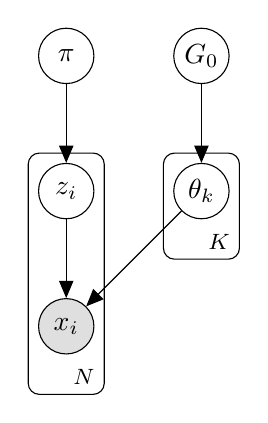
\begin{tikzpicture}

  % Define nodes
  \node[obs]                    (X) {$x_{i}$};
  \node[latent, above=of X] 	(Z) {$z_{i}$};
  \node[latent, above=of Z]  	(p) {$\pi$};
  \node[latent, right=1cm of Z] (t) {$\theta_{k}$};
  \node[latent, above=of t] 	(G) {$G_{0}$};

  % Connect the nodes
  \edge {Z,t} {X} ; %
  \edge {p} {Z} ; %
  \edge {G} {t} ; %

  % Plates
  \plate {} {(t)} {$K$};
  \plate {} {(Z)(X)} {$N$};

\end{tikzpicture}
%\endpgfgraphicnamed

%%% Local Variables: 
%%% mode: tex-pdf
%%% TeX-master: "example"
%%% End: 

	\emph{Graphical Model of FDMM.}
  \end{center}
\end{minipage}
%\hfill
\begin{minipage}{0.1\textwidth}%\raggedright
  \begin{equation*}
  	\begin{aligned}
  		\mathbf{\pi} \; & \sim \; Dir(\mathbf{\delta}) \\
  		z_{i}|\mathbf{\pi} \; & \sim \; Cat(\mathbf{\pi}) \\
  		\theta_{k} \; & \sim \mathcal{G}_{0}; \mathcal{H} \\
  		x_{i}|z_{i}=k,\theta_{k} \; & \sim \; p(\cdot | \theta_{k})  
  	\end{aligned} 
  \end{equation*} 
\end{minipage}

\vspace*{5mm}
The full joint distribution of the FDMM model by looking at the graphical representation factorizes as follows:
\begin{equation}%\scriptstyle
	p(\mathbf{X},\mathbf{Z},\mathbf{\pi},\Theta;\delta,\mathcal{H}) = p(\mathbf{X}|\mathbf{Z},\Theta) p(\mathbf{Z}|\pi) p(\pi|\delta) p(\Theta |\mathcal{G}_{0}; \mathcal{H})
\end{equation}

where $\mathcal{H}$ is the set of all the hyper-parameters of the $\mathcal{G}_{0}$ prior distribution related to the parameters $\Theta$, and $\mathbf{\delta}$ is a K-dimensional vector with the hyper-parameters of the \emph{Dirichlet} prior. 

To do inference in the Bayesian framework, the posterior distribution of the parameters needs to be computed. By applying the Bayes Rule and conditioning on the observed data $\mathbf{X}$, the posterior distribution is simply proportional to the full joint. Thus:
 
\begin{equation}%\scriptstyle
  \begin{aligned}
	p(\mathbf{Z},\mathbf{\pi},\Theta|\mathbf{X} ;\delta,\mathcal{H}) & = \frac{p(\mathbf{X}|\mathbf{Z},\mathbf{\pi},\Theta) p(\mathbf{Z},\mathbf{\pi},\Theta ;\delta,\mathcal{H})}{p(\mathbf{X})} \\
	   & \propto p(\mathbf{X}|\mathbf{Z},\mathbf{\pi},\Theta) p(\mathbf{Z},\mathbf{\pi},\Theta ;\delta,\mathcal{H}) \\
	   & = p(\mathbf{X}|\mathbf{Z},\Theta) p(\mathbf{Z}|\pi) p(\pi|\delta) p(\Theta |\mathcal{G}_{0}; \mathcal{H}) \\
	   & = \bigg(\prod\limits_{i=1}^{N} p(x_{i}|z_{i},\theta_{z_{i}}) p(z_{i}|\pi)\bigg) p(\pi|\delta) \bigg(\prod\limits_{k=1}^{K} p(\theta_{k} |\mathcal{G}_{0}; \mathcal{H})\bigg)
  \end{aligned}
\end{equation}
where we use the fact that $\mathbf{X}$ is conditionally independent of $\pi$ given $\mathbf{Z}$, \ie $\mathbf{X} \bigCI \pi \;| \; \mathbf{Z} $. 


Deriving Gibbs sampler for this model requires deriving an expression for the conditional distribution of every random variable conditioned on all the others. More specifically, for the FDMM we have the following quantities:
\begin{equation}%\scriptstyle
	p(\mathbf{\pi}|\mathbf{X},\mathbf{Z},\Theta;\delta,\mathcal{H}) = p(\mathbf{\pi} | \mathbf{Z};\delta) \sim Dir(\delta + N_{k})
\end{equation}

\begin{equation}%\scriptstyle
	p(\mathbf{\Theta}|\mathbf{X},\mathbf{Z},\pi;\delta,\mathcal{H}) = p(\mathbf{\Theta}|\mathbf{X},\mathbf{Z};\mathcal{H}) \sim \mathcal{G}_{0}(\cdot|\mathcal{H})
\end{equation}

\begin{equation}%\scriptstyle
	p(\mathbf{Z}|\mathbf{X},\mathbf{\Theta},\pi;\delta,\mathcal{H}) = p(\mathbf{\Theta}|\mathbf{X},\mathbf{Z};\mathcal{H}) \sim \mathcal{G}_{0}(\cdot|\mathcal{H})
\end{equation}
%\chapter{Mixture Modelling of DNA Methylation Profiles} \label{model-meth-chapter}

\section{Introduction} \label{motivation-meth-l}
DNA methylation data generated from NGS provide us with the methylation level of the genomic DNA at each cytosine. But, what is often of practical interest is identifying the methylation profile of a genomic region, \eg the methylation profile of a promoter. \cite{Vanderkraats2013} suggested that the shape of the methylation profile plays an important role in predicting gene expression, leading to a potentially functional role for methylation patterns. This means that higher-order properties, such as shape, of the methylation profiles over a region should be considered. Taking into consideration that the methylation level of a CpG site is highly correlated with the methylation level of the surrounding CpGs (\ie spatial co-dependence), \cite{Mayo2014} developed M$^3$D, which is non-parametric kernel-based method for statistical identification of differentially methylated regions (DMRs). This project makes the same assumption about the \emph{spatial co-dependence} of CpGs, but is mainly concentrated in clustering together similar methylation profiles.
\section{Modelling DNA Methylation Profiles} \label{model-meth-profiles-s}
The measurement process of DNA methylation can be modelled with a Binomial distribution. Assume that \emph{t} is the total number of reads that are mapped to a specific CpG site, and that the 5-Methylcytosine were found in \emph{m} of these reads. Then for each CpG site we have the read proportion \emph{(m,t)}, and we assume that:
\begin{equation} \label{binom-1d-f-meth}
	m \sim Binom(t, p)
\end{equation}
where \emph{p} is the unknown methylation level of the CpG site.

We are interested in modelling methylation profiles across different genomic regions, \eg promoter regions, hence the data can be represented as a set of vectors, whose dimensionality \emph{L} depends on the number of the individual CpG sites for that specific region. Formally, each region \emph{i} can be represented by a vector $\mathbf{y}_{i}$ of dimensionality $L_{i}$, and each entry of the vector consists of the tuple:
\begin{equation}
	%n_{i}^{l} = \frac{m_{i}^{l}}{t_{i}^{l}}
	y_{il} = (m_{il},t_{il})
\end{equation}
where, $m_{il}$ is the number of 5-Methylcytosine reads on $l$-th CpG site in region $i$, and $t_{il}$ is the total number of reads on $l$-th CpG site in region $i$. 

Hence, we can formulate our problem as a \emph{regression} problem, where we try to fit a function $\mathbf{f}$, of some specific form, to the observations $\mathbf{y}$. A promising approach for modelling the methylation profile for a given region is to use a \emph{Gaussian Process} for classification \citep{Rasmussen2006}. Even though this approach would be ideal, its time complexity of $O(n^{3})$ is prohibitive for our purposes. A computationally more attractive approach would be to follow a parametric approach by selecting an explicit set of basis functions.

More specifically, let $\mathbf{x}_{i}$ be the genomic region of interest, $\mathbf{y}_{i}$ be the vector of observations in this region (\ie proportions of methylated reads to the total reads at each site), and let $f(\mathbf{x}_{i})$ be a latent function representing the methylation profile at that specific genomic region. Since the observed methylation data are actually the fraction of total reads that contained methylated cytosines, each entry in the region will take values in the $[0, 1]$ interval, thus, we introduce a latent function $g(\mathbf{x}_{i})$, \eg $g(\mathbf{x}_{i}) = \alpha \mathbf{x}_{i}^{2} + \beta \mathbf{x}_{i} + c$, defined as the \emph{inverse probit transformation} of $f(\mathbf{x}_{i})$. In other words, $f(\mathbf{x}_{i})$ is the probit transformation of $g(\mathbf{x}_{i})$:
\begin{equation} \label{probit-transform-f-meth}
	f(\mathbf{x}_{i}) = \Phi(g(\mathbf{x}_{i}))
\end{equation}
where $\Phi(x)$ is the Cumulative Distribution Function (CDF) of the standard normal distribution:
\begin{equation} \label{cdf-stand-normal-f-meth}
	\Phi(x) = \frac{1}{\sqrt{2\pi}} \int_{-\infty}^{x} e^{-t^{2}/2}dt
\end{equation}

Let $\mathbf{f}_{i} = f(\mathbf{x}_{i})$ and $\mathbf{g}_{i} = g(\mathbf{x}_{i})$ be shorthand for the values of the latent functions.

Given the values of the latent function $\mathbf{f}_{i}$, the observations at each CpG site for that region are independent Binomial variables, as shown in \emph{Eq. \ref{binom-1d-f-meth}}, so the joint likelihood factorizes and we have:
\begin{equation} \label{likel-binom-prob-f-meth}
  \begin{split}
	p(\mathbf{y}_{i}|\mathbf{f}_{i}) & = \prod_{l=1}^{L} p(y_{il}|f_{il}) \\
							 & = \prod_{l=1}^{L} Binom(t_{il}, f_{il}) \\
							 & = \prod_{l=1}^{L} Binom\big(t_{il}, \Phi(g_{il})\big) \\
							 & = \prod_{l=1}^{L} \binom{t_{il}}{m_{il}} \Phi(g_{il})^{m_{il}} (1 - \Phi(g_{il})\big)^{t_{il} - m_{il}}
  \end{split}
\end{equation}

From its final form, we refer to this function as the \emph{Binomial distributed Probit regression function}. In practice, the likelihood is computed in the log space, due to numerical issues when multiplying many probabilities of small numbers leading to underflow errors. Thus, the joint log likelihood for region \emph{i} is:
\begin{equation} \label{likel-binom-prob-log-f-meth}
  \begin{split}
	\log p(\mathbf{y}_{i}|\mathbf{f}_{i}) & = \sum_{l=1}^{L} \log p(y_{il}|f_{il}) \\
				& = \sum_{l=1}^{L} \log \bigg(\binom{t_{il}}{m_{il}} \Phi(g_{il})^{m_{il}} \big(1 - \Phi(g_{il})\big)^{t_{il} - m_{il}}\bigg) \\
				& = \sum_{l=1}^{L} \bigg(\log \binom{t_{il}}{m_{il}} + m_{il} \log \Phi(g_{il}) + \big(t_{il} - m_{il} \big) \log \big(1 - \Phi(g_{il})\big)\bigg)
  \end{split}
\end{equation}
\section{Clustering DNA Methylation Profiles} \label{cluster-meth-s}
After defining a model for the DNA methylation profiles, a statistical method needs to be proposed in order to perform model-based clustering of methylation profiles. 

A mixture model approach \citep{McLachlan1988} is chosen to cluster methylation profiles, and the model is fitted to the data using maximum likelihood. Thus, \emph{EM algorithm} \citep{Dempster1977} is chosen to estimate the mixture model parameters. Below we derive the \emph{E} and \emph{M} steps for clustering methylation profiles using the \emph{Binomial distributed Probit regression function} as the observation model. 

But before, we have to explicitly introduce the parameters $\theta_{k}$ of the observation model, excluding the mixing proportions $\pi_{k}$ which are present for any mixture model. For example, in a Gaussian Mixture Model (GMM) the model parameters $\theta_{k}$ are the mean $\mu_{k}$ and the variance $\sigma_{k}^{2}$ of the Gaussian components. In our model, the Binomial distributed Probit regression function, the parameters are the coefficients of the $n^{th}$ degree polynomial function $\mathbf{g}_{i}$. Thus, during the EM algorithm we infer these sets of parameters for each cluster $k$. 

For example, for a $2^{nd}$ degree polynomial, we can rewrite \emph{Eq. \ref{likel-binom-prob-f-meth}} by explicitly showing the model parameters as follows:
\begin{equation} \label{likel-binom-prob-example1-f-meth}
  \begin{split}
	p(\mathbf{y}_{i}|\mathbf{f}_{i}, \theta) & = \prod_{l=1}^{L} p(y_{il}|f_{il}, \theta) \\
							 & = \prod_{l=1}^{L} Binom \big(t_{il}, \Phi(g_{il}; \theta)\big) \\
							 & = \prod_{l=1}^{L} \binom{t_{il}}{m_{il}} \Phi(\alpha x_{il}^{2} + \beta x_{il} + c)^{m_{il}} (1 - \Phi(\alpha x_{il}^{2} + \beta x_{il} + c)\big)^{t_{il} - m_{il}}
  \end{split}
\end{equation}
where $\theta = (\alpha, \beta, c)$.

\subsection{E-step}
In the E-step we compute the responsibility that component k takes on explaining observations $\mathbf{y}_{i}$, and by substituting the proposed likelihood function to \emph{Eq. \ref{responsibilities-f-mm}}, we have:
\begin{equation} \label{responsibilities-binom-prob-model-f-meth}
  \begin{split}
	\gamma(z_{ik}) & \triangleq p(z_{i}=k|\mathbf{y}_{i},\theta_{k}) \\
				   & = \frac{\pi_{k}p(\mathbf{y}_{i}|\mathbf{f}_{i},z_{i}=k,\theta_{k})}{\sum\limits_{j=1}^{K} \pi_{j}p(\mathbf{y}_{i}|\mathbf{f}_{i},z_{i}=j,\theta_{j})} \\
				   & = \frac{\pi_{k} \prod\limits_{l=1}^{L} Binom \big(t_{il}, \Phi(g_{il}; \theta_{k})\big)} {\sum\limits_{j=1}^{K} \pi_{j} \prod\limits_{l=1}^{L} Binom \big(t_{il}, \Phi(g_{il}; \theta_{j})\big)}
  \end{split}
\end{equation}
Thus, the E-step essentially remains the same, with the difference that at each iteration we need to evaluate pointwise a different observation model. 

\subsection{M-step}
In the M-step, we need to optimize \emph{Eq. \ref{log-lik-expected-derivation-f-mm}} with respect to $\pi_{k}$ and $\theta_{k}$. The update for the mixing proportions $\pi_{k}$ for each M-step remains the same as the simple mixture model, that is:
\begin{equation} \label{mixing-proportions-binom-prob-est-f-meth}
		\pi_{k} = \frac{1}{N} \sum_{i} \gamma(z_{ik})
\end{equation}

To update the parameters $\theta_{k}$, we need to optimize the following quantity:
\begin{equation} \label{parameters-est2-binom-prob-EM-f-meth}
  \begin{split}
	\ell(\theta_{k}) & \triangleq \sum_{i} \sum_{k} \gamma(z_{ik}) \log p(\mathbf{y}_{i}|\mathbf{f}_{i}, \theta_{k}) \\
					 & = \sum_{i} \sum_{k} \gamma(z_{ik}) \log \bigg( \prod_{l} Binom \big(t_{il}, \Phi(g_{il}; \theta_{k})\big) \bigg)\\
					 & = \sum_{i} \sum_{k} \gamma(z_{ik}) \sum_{l} \log \bigg(Binom \big(t_{il}, \Phi(g_{il}; \theta_{k})\big) \bigg)
  \end{split}
\end{equation}

Direct maximization of this quantity w.r.t the parameters $\theta_{k}$ is not feasible, thus Conjugate Gradients method \citep{Hestenes1952} will be used, which is a first order numerical optimization algorithm for solving particular systems of linear equations. Hence, it requires to compute the \emph{gradient}, which for the example of the $2^{nd}$ degree polynomial is:

\begin{equation} \label{gradient-f}
	\nabla\ell = \bigg( \frac{\partial \ell(\theta_{k})}{\partial \alpha}, \frac{\partial \ell(\theta_{k})}{\partial \beta}, \frac{\partial \ell(\theta_{k})}{\partial c}\bigg) 
\end{equation}
where the partial derivatives are given in the equations below (see \emph{Appendix \ref{derivatives-m-step-chapter}} for the whole derivations):
\begin{equation} \label{derivative-a-f}
	\frac{\partial \ell(\theta_{k})}{\partial \alpha} =  \sum_{i}  \gamma(z_{ik}) \sum_{l} \bigg[ x_{il}^{2} \mathbf{\phi}(g_{il};\theta_{k})\bigg(\frac{m_{il} - t_{il}\Phi(g_{il};\theta_{k})}{\Phi(g_{il};\theta_{k})\big(1-\Phi(g_{il};\theta_{k})\big)} \bigg) \bigg]
\end{equation}

\begin{equation} \label{derivative-b-f}
	\frac{\partial \ell(\theta_{k})}{\partial \beta} =  \sum_{i}  \gamma(z_{ik}) \sum_{l} \bigg[ x_{il} \mathbf{\phi}(g_{il};\theta_{k})\bigg(\frac{m_{il} - t_{il}\Phi(g_{il};\theta_{k})}{\Phi(g_{il};\theta_{k})\big(1-\Phi(g_{il};\theta_{k})\big)} \bigg) \bigg]
\end{equation}

\begin{equation} \label{derivative-c-f}
	\frac{\partial \ell(\theta_{k})}{\partial c} =  \sum_{i}  \gamma(z_{ik}) \sum_{l} \bigg[ \mathbf{\phi}(g_{il};\theta_{k})\bigg(\frac{m_{il} - t_{il}\Phi(g_{il};\theta_{k})}{\Phi(g_{il};\theta_{k})\big(1-\Phi(g_{il};\theta_{k})\big)} \bigg) \bigg]
\end{equation}
where $\mathbf{\phi}$ is the \emph{probability density function} for the standard normal distribution $\mathcal{N}(0,1)$.

\subsection{EM initialization}
EM algorithm is sensitive to the choice of the initial parameters. Thus, careful initialization would result in faster convergence to local maximum or even in finding better local maxima. When using simple mixture models, like GMMs, the parameters themselves have physical interpretation, \eg the mean value of the data, thus \emph{k-means} algorithm can be used directly on the observation data to initialize the parameters.

The model proposed in this work, is more complex since each object is a vector of observations, and these vectors may also be of different length. To provide a sensible initialization of the parameters, the following procedure is taken:
\begin{itemize}
	\item{For each object, we fit a latent function to its observations using \emph{Conjugate Gradients} algorithm to obtain a coefficient vector of the polynomial.}
	\item{After extracting all the coefficient vectors for each object, we run \emph{k-means} on them. The output of \emph{k-means}, will be the initial values for the model parameters.}
\end{itemize}

\section{Experiments} \label{meth-experiments-sect}

\section{Synthetic Experiments} \label{meth-synth-experiments-sect}

\input{Methylation/meth-synth-data}
\input{Methylation/meth-synth-eval}
\input{Methylation/meth-synth-model}
%\input{meth-exp}
%\include{rna-seq}
%\section{Bayesian Consensus Clustering} \label{bcc-sec-l}
Bayesian Consensus Clustering can be thought as an extension of a mixture model so as to account for multiple data sources. Thus, before explaining the BCC model the Dirichlet Mixture Model (DMM) will be described, which will put the groundwork in having a better understanding of the integrative model.

The mixture model was described in \emph{Section \ref{cluster-meth-l}}. Under a Bayesian framework the Dirichlet Mixture Model arises, where the parameters themselves are considered as random variables, thus prior distributions will be placed over the random variables. 

If possible, conjugate priors should be used since the posterior distributions will be in the same family as the prior probability distributions. Thus, a natural choice is to use a Dirichlet prior distribution for the mixing proportions $\Pi$. For the parameters $\Theta$, appropriate priors should be chosen depending on the probability distributions that the data follow.

\emph{Figure \ref{fdmm-pic}} shows a graphical representation of the DMM, where $G_{0}$ is the prior probability distribution for the parameters $\theta_{k}$.

% DMM model
\begin{figure}[ht]
  \begin{center}
      % model_pca.tex
%
% Copyright (C) 2012 Jaakko Luttinen
%
% This file may be distributed and/or modified
%
% 1. under the LaTeX Project Public License and/or
% 2. under the GNU General Public License.
%
% See the files LICENSE_LPPL and LICENSE_GPL for more details.

% PCA model

%\beginpgfgraphicnamed{model-pca}
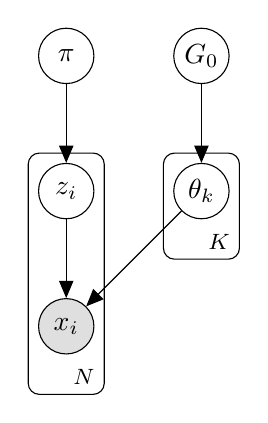
\begin{tikzpicture}

  % Define nodes
  \node[obs]                    (X) {$x_{i}$};
  \node[latent, above=of X] 	(Z) {$z_{i}$};
  \node[latent, above=of Z]  	(p) {$\pi$};
  \node[latent, right=1cm of Z] (t) {$\theta_{k}$};
  \node[latent, above=of t] 	(G) {$G_{0}$};

  % Connect the nodes
  \edge {Z,t} {X} ; %
  \edge {p} {Z} ; %
  \edge {G} {t} ; %

  % Plates
  \plate {} {(t)} {$K$};
  \plate {} {(Z)(X)} {$N$};

\end{tikzpicture}
%\endpgfgraphicnamed

%%% Local Variables: 
%%% mode: tex-pdf
%%% TeX-master: "example"
%%% End: 

  \caption{Graphical representation of the Dirichlet Mixture Model.}
  \label{fdmm-pic}
  \end{center}
\end{figure}

To perform integrative clustering from M different data sources $\mathbb{X}_{1},..., \mathbb{X}_{M}$, the DMM model is extended which leads us to the Bayesian Consensus Clustering (BCC) model \cite{Lock2013}. BCC model assumes that there are N common objects for each data source, where $X_{mn}$ denotes the data for object $n$ from source $m$.
The model is very general and the data sources $\mathbb{X}_{m}$ can have any disparate structure, and each of them requires an arbitrary probability model $f_{m}(X_{mn}|\theta_{m})$.

Let $\mathbb{L}_{m} = (L_{m1},...,L_{mN})$ denote the source specific clusterings and $\mathbb{C} = (C_{1},...,C_{N})$ denote the overall clustering of the data. The model assumes that both $\mathbb{C}$ and $\mathbb{L}_{m}$ will have the same number of possible clusters K, thus $L_{mn} \in \lbrace 1,...,K \rbrace$ and $C_{n} \in \lbrace 1,...,K \rbrace$, will denote the source specific and the overall mixture component for observation $X_{mn}$, respectively.

The source specific clusterings and the overall clustering are related to each other, and the strength of the relation is given by a dependence function $v(L_{mn}, C_{n}, \alpha_{m})$, where $\alpha_{m} \in [\frac{1}{K}, 1]$ is the adherence parameter and controls the adherence of data source $\mathbb{X}_m$ to the overall clustering $\mathbb{C}$. More simply, it explains how much does the source specific clustering for source $m$ agrees with the overall clustering $\mathbb{C}$. So if $\alpha_{m} = 1$, then $\mathbb{L}_{m} = \mathbb{C}$. 

The dependence function $v$ has the form:

\begin{equation}
	v(L_{mn}, C_{n}, \alpha_{m}) = \left\{
	\begin{array}{l l}
		\alpha_{m},\quad \quad \quad if\quad C_{n} = L_{mn}\\
		\frac{1-\alpha_{m}}{K-1},\quad \quad otherwise
	\end{array}\right.
\end{equation}

The graphical representation for the BCC model is given in \emph{Figure \ref{bcc-pic}}, where again $G_{0}$ is the prior for the parameters $\theta_{mk}$.

% BCC model
\begin{figure}[ht]
  \begin{center}
      % model_pca.tex
%
% Copyright (C) 2012 Jaakko Luttinen
%
% This file may be distributed and/or modified
%
% 1. under the LaTeX Project Public License and/or
% 2. under the GNU General Public License.
%
% See the files LICENSE_LPPL and LICENSE_GPL for more details.

% PCA model

%\beginpgfgraphicnamed{model-pca}
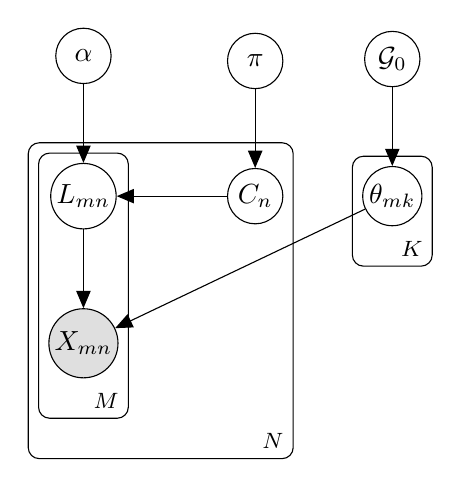
\begin{tikzpicture}

  % Define nodes
  \node[obs]                              (X) {$X_{mn}$};
  \node[latent, above=of X] 		(L) {$L_{mn}$};
  \node[latent, above=of L] 		(a) {$\alpha$};
  \node[latent, right=1.4cm of L]  (C) {$C_{n}$};
  \node[latent, above=of C] 		(p) {$\pi$};
  \node[latent, right=1cm of C]  (t) {$\theta_{mk}$};
  \node[latent, above=of t] 		(G) {$\mathcal{G}_{0}$};

  % Connect the nodes
  \edge {L,t} {X} ; %
  \edge {a,C} {L} ; %
  \edge {p} {C} ; %
  \edge {G} {t} ; %

  % Plates
  \plate {} {(t)} {$K$};
  \plate {yx} {(L)(X)} {$M$};
  \plate {} {(C)(X)(yx.north west)(yx.south west)} {$N$};

\end{tikzpicture}
%\endpgfgraphicnamed

%%% Local Variables: 
%%% mode: tex-pdf
%%% TeX-master: "example"
%%% End: 

  \caption{Graphical representation of Bayesian Consensus Clustering.}
  \label{bcc-pic}
  \end{center}
\end{figure}

The full joint distribution of the model by looking at the graphical representation in \emph{Fig \ref{bcc-pic}} is given by:

\begin{equation}\scriptstyle
	P(\mathbb{X}, \mathbb{L}, \mathbb{C}, \Pi , \Theta , \alpha ; \mathcal{H}) = P(\mathbb{X}|\mathbb{L},\Theta) P(\mathbb{L}|\mathbb{C},\alpha) P(\mathbb{C}|\Pi) P(\Pi) P(\alpha) P(\Theta ; \mathcal{H})
\end{equation}

where $\mathcal{H}$ is the set of all the hyper-parameters, related to the parameters $\Theta$. 

To do inference in the Bayesian framework, the posterior distribution of the parameters needs to be computed. By applying the Bayes Rule and conditioning on the observed data $\mathbb{X}$, the posterior distribution is simply proportional to the full joint. Thus:
 
\begin{equation}\scriptstyle
	\begin{aligned}
	& & \scriptstyle P(\mathbb{L},\mathbb{C},\Pi ,\Theta , \alpha | \mathbb{X}; \mathcal{H}) & \scriptstyle \propto P(\mathbb{X}|\mathbb{L}, \mathbb{C},\Pi ,\Theta , \alpha) P(\mathbb{L}, \mathbb{C}, \Pi , \Theta , \alpha; \mathcal{H}) \\
	& & & \scriptstyle = P(\mathbb{X}|\mathbb{L},\Theta) P(\mathbb{L}|\mathbb{C},\alpha) P(\mathbb{C}|\Pi) P(\Pi) P(\alpha) P(\Theta ; \mathcal{H})
	\end{aligned}
\end{equation}

This posterior is intractable to compute, thus we need to resort to approximation schemes and these fall broadly into two classes. Deterministic approximation schemes such as \emph{variational inference} could be used, which are based on analytically approximating the posterior distribution, by assuming that it factorizes in a particular way, or that the posterior will have a specific parametric form, such as a Gaussian, which then we try to approximate.

The other approximation scheme, and the one that is used in this project, is a stochastic approximation of the posterior using Markov Chain Monte Carlo (MCMC) methods. Specifically, \emph{Gibbs sampling} algorithm will be used, which is one of the most popular MCMC algorithms. 

Deriving Gibbs sampling for this model, requires deriving an expression for the \emph{full conditional distribution} of every latent variable conditioned on all the others. Thus, from the graphical model shown in \emph{Figure \ref{bcc-pic}}, we can infer the dependencies of the latent variables by looking at the \emph{Markov blanket} of each variable, which are its neighbours in the graph. 

For mathematical convenience, \emph{conjugate priors} should be used which would allow us to perform analytically some marginalization steps that are necessary in deriving Gibbs sampler. Thus:

\begin{itemize}
	\item $\Pi \sim Dir(\mathbf{\delta_{0}})$. For the mixing proportions a natural choice is a Dirichlet prior distribution, and the hyper-parameter vector $\mathbf{\delta_{0}}$ is set to $(1,...,1)$ so the prior is uniformly distributed in the $K-1$ simplex.
	\item $\alpha_{m} \sim TBeta(\mathit{a_{m}}, \beta_{m}, \frac{1}{K})$. Which means that $a_{m}$ follows a  $Beta$ distribution with parameters $\mathit{a_{m}}, \beta_{m}$ truncated below by $\frac{1}{K}$.
	\item $\theta_{mk} \sim G_{0}$. Where $G_{0}$ is a conjugate prior distribution so that sampling from the conditional posterior $p_{m}(\theta_{mk}|\mathbb{X}_{m}, \mathbb{L}_{m})$ is feasible. For example, if the probability model $f_{m}(X_{mn}|\theta_{m}) \sim Poisson(\lambda_{m})$, then a conjugate prior distribution would be a $Gamma(\lambda_{m}|\mathit{a_{m}}, \beta_{m})$.
\end{itemize}

Having chosen the appropriate prior distributions, the Gibbs sampler would proceed iteratively by sampling from the following full conditional distributions:

\begin{enumerate}
	\item $\scriptstyle \mathbb{L}_{m} | \mathbb{X}_{m}, \Theta_{m}, \mathbb{C}, \alpha_{m} \sim v(L_{mn}, C_{n}, \alpha_{m}) f_{m}(X_{mn}|\theta_{mk}) \quad \text{for} \quad n=1,...,N $
	\item $\scriptstyle \Theta_{m}|\mathbb{L}_{m}, \mathbb{X}_{m} \sim p_{m}(\theta_{mk}|\mathbb{X}_{m}, \mathbb{L}_{m}) \quad \text{for} \quad k=1,...,K $
	\item $\scriptstyle \alpha_{m}|\mathbb{L}_{m}, \mathbb{C} \sim TBeta \big(\mathit{a_{m}}+\sum_{n=1}^{N}\mathbbm{1}(L_{mn}=k,C_{n}=k), \beta_{m}-N-\sum_{n=1}^{N}\mathbbm{1}(L_{mn}=k,C_{n}=k), \frac{1}{K}\big)$
	\item $\scriptstyle \mathbb{C}|\mathbb{L}_{m}, \Pi, \alpha \sim \pi_{k}\prod_{m=1}^{M}v(L_{mn, C_{n}, \alpha_{m}}) \quad \text{for} \quad n=1,...,N$
	\item $\scriptstyle \Pi|\mathbb{C} \sim Dirichlet(\{ \delta_{k} + \sum_{n=1}^{N}\mathbbm{1}(C_{n}=k)\}_{k=1}^{K })$
\end{enumerate}
%\chapter{Discussion} \label{discussion-chapter}

%\section{Introduction} \label{data-intro-sect}
This chapter is concerned with introducing data generated from Next Generation Sequencing (NGS) technology, also termed as high-throughput sequencing. \emph{DNA sequencing} is the process of determining the complete order of DNA nucleotides of an organism's genome at a single time. Until recently, the method of choice for DNA sequencing was the \emph{chain termination} method developed by \citet{Sanger1977}. This technology, and its variants, even though they were widely adopted, they had inherent limitations in throughput, scalability, speed and cost. 

NGS technology \citep{Shendure2008, Mardis2008}, performs massively parallel sequencing on DNA fragments, producing thousands or millions of DNA fragment sequences, called \emph{reads}, concurrently. This yields substantially higher throughput and allows for entire genomes to be sequenced within a day. By reducing the cost by over two orders of magnitude from traditional Sanger sequencing methods \citep{Shendure2008}, DNA sequencing became accessible for smaller labs, allowing for rapid development of applications in fields related to biological and biomedical sciences. Even though, millions of biological data are generated from NGS technology, computational data analysis is still a challenging task.


%%%%%%%%
%% Any appendices should go here. The appendix files should look just like the
%% chapter files.
\appendix
\chapter{Partial derivatives for M-step} \label{derivatives-m-step-s}

We need to compute the partial derivatives w.r.t. parameters $\theta_{k}$ of the following quantity:
\begin{equation} \label{parameters-est2-EM-f-app}
  \begin{split}
	\ell(\theta_{k}) & \triangleq \sum_{i} \sum_{k} \gamma(z_{ik}) \log p(\mathbf{y}_{i}|\mathbf{f}_{i}, \theta_{k}) \\
					 & = \sum_{i} \sum_{k} \gamma(z_{ik}) \sum_{l} \log \bigg(Binom \big(t_{il}, \Phi(g_{il}; \theta_{k})\big) \bigg) \\
					 & \propto  \sum_{i} \sum_{k} \gamma(z_{ik}) \sum_{l} \bigg(m_{il} \log \Phi(g_{il}; \theta_{k}) + \big(t_{il} - m_{il} \big) \log \big(1 - \Phi(g_{il}; \theta_{k})\big)\bigg)
  \end{split}
\end{equation}
where $\theta_{k} = (\alpha, \beta, c)$ in the example of $2^{nd}$ degree polynomial, i.e. $g_{il} = \alpha x^{2} + \beta x + c$. To not clutter notation, let $\Phi(g_{il}) = \Phi(g_{il}; \theta_{k})$. Thus, for the partial derivatives w.r.t. $\alpha$ parameter we have the following derivation:

\begin{equation} \label{derivative-a-f-app}
  \begin{split}
	\frac{\partial \ell(\theta_{k})}{\partial \alpha} & = \sum_{i} \gamma(z_{ik}) \sum_{l} \bigg[ m \frac{\partial}{\partial \alpha}\big(\log \Phi(g_{il})\big) + (t-m) \frac{\partial}{\partial \alpha}\big(\log \big[1 - \Phi(g_{il})\big]\big)\bigg] \\
		& = \sum_{i} \gamma(z_{ik}) \sum_{l} \bigg[ \frac{m}{\Phi(g_{il})} \frac{\partial \Phi(g_{il})}{\partial g_{il}} \frac{\partial g_{il}}{\partial \alpha} + \frac{t - m}{1 - \Phi(g_{il})}\bigg( -\frac{\partial \Phi(g_{il})}{\partial g_{il}} \frac{\partial g_{il}}{\partial \alpha} \bigg) \bigg] \\
		& = \sum_{i} \gamma(z_{ik}) \sum_{l} \bigg[ \frac{m}{\Phi(g_{il})} x_{il}^{2} \mathbf{\phi}(g_{il}) - \frac{t - m}{1 - \Phi(g_{il})} x_{il}^{2} \mathbf{\phi}(g_{il}) \bigg]\\
		& = \sum_{i}  \gamma(z_{ik}) \sum_{l} \bigg[ x_{il}^{2} \mathbf{\phi}(g_{il})\bigg(\frac{m}{\Phi(g_{il})} - \frac{t - m}{1 - \Phi(g_{il})}\bigg) \bigg] \\
		& = \sum_{i}  \gamma(z_{ik}) \sum_{l} \bigg[ x_{il}^{2} \mathbf{\phi}(g_{il})\bigg(\frac{m_{il} - t_{il}\Phi(g_{il})}{\Phi(g_{il})\big(1-\Phi(g_{il})\big)} \bigg) \bigg]
	\end{split}
\end{equation}
where $\mathbf{\phi}(g_{il}) \triangleq \mathbf{\phi}(g_{il};\theta_{k})$ is the \emph{probability density function (pdf)} for the standard normal distribution $\mathcal{N}(0,1)$.

In a similar fashion we can derive the partial derivatives $\frac{\partial \ell(\theta_{k})}{\partial \beta}$ and $\frac{\partial \ell(\theta_{k})}{\partial c}$.




\chapter{Poisson mixture model for NGS data}
Let $\mathbf{x}=x_{ijl}$ be the gene expression data for object (\ie gene) $i \;(i = 1,...,N)$ of condition $j \; (j=1,...,D)$ in biological replicate $l \; (l=1,...,r_{j})$. To cluster together co-expressed genes a Poisson mixture model is used. This model is parametrized to account for specific characteristics of RNA-Seq data, including:
(1) an offset parameter $w_{i}$ which corresponds to the overall expression level of observation $i$, \ie $w_{i} = \sum\limits_{j}\sum\limits_{l} x_{ijl}$, (2) a normalization factor $s_{jl}$ to account for different library sizes and (3) an unknown parameter $\lambda_{jk}$ which corresponds to the proportion of reads attributed to condition $j$ in cluster $k$. The $w_{i}$ and $s_{jl}$ are estimated from the data prior to fitting the model, and thus are considered to be fixed.

Assuming the samples are conditionally independent given the cluster components, the likelihood for the Poisson mixture model is given by:
\begin{equation} \label{poisson-log-lin-mm-app}
  \begin{split}
	\ell(\mathbf{\lambda}) \triangleq p(\mathbf{x} | \mathbf{\lambda}) & = \sum\limits_{z} p(\mathbf{z}) p(\mathbf{x} | \mathbf{\lambda}, \mathbf{z})\\
		& = \prod_{i} \sum_{k} p(z_{i} = k) \prod_{j} \prod_{l} \mathcal{P}(x_{ijl} | \mu_{ijlk}) \\
		& = \prod_{i} \sum_{k} \pi_{k} \prod_{j} \prod_{l} \mathcal{P}(x_{ijl} | w_{i}s_{jl} \lambda_{jk})
  \end{split}
\end{equation}
where $\mathcal{P}(\cdot)$ denotes the Poisson probability mass function, $w_{i}$ and $s_{jl}$ are considered to be fixed constants learned from the data, and $\mathbf{z}$ are discrete \emph{latent variables} representing from which cluster each object was generated. 

For a specific condition $j$ in cluster $k$, the likelihood function simplifies to:
\begin{equation} \label{poisson-log-lin-mm-jk-app}
  \begin{split}
	\ell(\lambda_{jk}) & \triangleq \prod_{i} \bigg( \pi_{k} \prod_{l} \mathcal{P}(x_{ijl} | w_{i}s_{jl} \lambda_{jk})\bigg)^{\mathbb{I}(z_{i}=k)}
  \end{split}
\end{equation}

In the Bayesian framework we need to define prior distributions on the parameters and if possible \emph{conjugate priors}. For the parameter of the Poisson probability mass function a natural choice is to use a Gamma prior:
\begin{equation} \label{poisson-prior-mm-app}
  \begin{split}
  \lambda_{jk} & \sim \mathcal{G}(\alpha, \beta) \\
  	& = \frac{\beta^{\alpha}}{\Gamma(\alpha)}\lambda_{jk}^{(\alpha-1)} e^{-(\lambda_{jk}\beta)}
    \end{split}
\end{equation}
where $\mathcal{G}(\alpha, \beta)$ denotes the Gamma probability distribution with \emph{shape} parameter $\alpha$ and \emph{rate} parameter $\beta$, and $\Gamma(\alpha)$ is the \emph{Gamma} function evaluated at $\alpha$.

Using the Bayes Rule, we can compute the posterior distribution for the parameter $\lambda_{jk}$ as follows:

\begin{equation} \label{posterior-poisson-bayes-rule-app}
  \begin{split}
  	p(\lambda_{jk} | \mathbf{x}) & = \frac{p(\mathbf{x}| \lambda_{jk}) \times p(\lambda_{jk})}{p(\mathbf{x})} \\
  		& \propto p(\mathbf{x}| \lambda_{jk}) \times p(\lambda_{jk}) \\
  		& = \prod_{i} \bigg(\pi_{k} \prod_{l} \mathcal{P}(x_{ijl} | w_{i}s_{jl} \lambda_{jk})\bigg)^{\mathbb{I}(z_{i}=k)} \times \mathcal{G}(\lambda_{jk}|\alpha, \beta) \\
  		& = \prod_{i} \bigg(\pi_{k} \prod_{l} \frac{1}{x_{ijl}!} e^{-(w_{i}s_{jl}\lambda_{jk})} (w_{i}s_{jl}\lambda_{jk})^{x_{ijl}}\bigg)^{\mathbb{I}(z_{i}=k)} \times \frac{\beta^{\alpha}}{\Gamma(\alpha)}\lambda_{jk}^{(\alpha-1)} e^{-(\lambda_{jk}\beta)} \\
  		& \propto \prod_{i} \bigg( \prod_{l} \lambda_{jk}^{x_{ijl}} e^{-(w_{i}s_{jl}\lambda_{jk})}\bigg)^{\mathbb{I}(z_{i}=k)} \times \lambda_{jk}^{(\alpha-1)} e^{-(\lambda_{jk}\beta)} \\
  		& = \lambda_{jk}^{\big(\sum\limits_{i} \mathbb{I}(z_{i}=k) \sum\limits_{l} x_{ijl}\big)} e^{-\lambda_{jk}\big(\sum\limits_{i} \mathbb{I}(z_{i}=k) \sum\limits_{l} w_{i}s_{jl}\big)} \times \lambda_{jk}^{(\alpha-1)} e^{-(\lambda_{jk}\beta)} \\
		& = \lambda_{jk}^{\big(\sum\limits_{i} \mathbb{I}(z_{i}=k) \sum\limits_{l} x_{ijl} + a -1\big)} e^{-\lambda_{jk}\big(\sum\limits_{i} \mathbb{I}(z_{i}=k) \sum\limits_{l} w_{i}s_{jl} + \beta \big)}
  \end{split}
\end{equation}

This quantity is an unnormalized Gamma distribution, so the posterior is in the same family distribution as the prior and can be written as follows:
\begin{equation} \label{posterior-poisson-final-app}
  	p(\lambda_{jk} | \mathbf{x}) = \mathcal{G}\bigg(a + \sum\limits_{i} \mathbb{I}(z_{i}=k) \sum\limits_{l} x_{ijl}, b + \sum\limits_{i} \mathbb{I}(z_{i}=k) \sum\limits_{l} w_{i}s_{jl} \bigg)
\end{equation}
 



%% Choose your favourite bibliography style here.
\bibliographystyle{apalike}

%% If you want the bibliography single-spaced (which is allowed), uncomment the next line.
%% \singlespace

%% Specify the bibliography file.
\bibliography{library}

\end{document}